\documentclass{article}[11pt, a4paper, oneside]

\usepackage[ngerman]{babel} % neue deutsche Trennungsregeln, etc
\usepackage[hidelinks]{hyperref} % Hyperlinks ohne Umrandungen
\usepackage{setspace} % Abstände zwischen Absätzen
\usepackage[left=2cm, right=2cm, top=2cm, bottom=2cm]{geometry} % Seitenränder
\onehalfspacing % 1,5 Zeilenabstand
\usepackage{lipsum}  % Dummy-Texte
\usepackage{titlesec} % define size for section headings
\usepackage[nohyperlinks, printonlyused]{acronym} % Abkürzungen


%% 
%% Schriftarten und -größen
%%
\titleformat{\section}{\normalfont\fontsize{12pt}{1.5}\bfseries}{\thesection}{1em}{} % Überschriften
\usepackage{fontspec}
\setmainfont{Arial}
  
% automatischens Einrücken von Absätzen verhindern
\usepackage{changepage}
\setlength{\parindent}{0pt}
% 6pt Abstand nur zwischen Absätzen
\setlength{\parskip}{6pt}{}

% Grafiken einbinden
\usepackage{graphicx}       
\usepackage[utf8]{inputenc} % korrekte Darstellung von Umlauten

\def\UrlFont{\rm} % Print URLs not in Typewriter Font

%% Informationen für die PDF-Datei
\hypersetup{
 pdfauthor={Markus Haug},
 pdftitle={Meine Fallstudie}
 pdfsubject={Not set},
 pdfkeywords={Not set}
}

%%
%% Bibliographie
%%
\usepackage{csquotes}
\usepackage[style=apa]{biblatex}
\addbibresource{references.bib}


\newcommand{\blankpage}{% Leerseite ohne Seitennummer, nächste Seite rechts
 \clearpage{\pagestyle{empty}\cleardoublepage}
}

% https://stackoverflow.com/questions/28572590/latex-retake-page-numbering
\ExplSyntaxOn% http://tex.stackexchange.com/a/227859/5764
\DeclareExpandableDocumentCommand{\arabicnumeral}{m}
  {
  \int_from_roman:n { #1 }
  }
\ExplSyntaxOff

%% ++++++++++++++++++++++++++++++++++++++++++
%% Dokument
%% ++++++++++++++++++++++++++++++++++++++++++
\begin{document}
\pagenumbering{Roman} % Uppercase Roman numerals
%% Titelseite
\def\usesf{}
\let\usesf\sffamily % diese Zeile auskommentieren für normalen TeX Font

\newsavebox{\Tutorin}
\savebox{\Tutorin}{<Name des Tutors>}


\setlength{\unitlength}{1pt}

\begin{titlepage}
%\vspace*{-39pt}\hspace*{300pt}\includegraphics[width=.27\paperwidth]{logos/IOSB}
\vspace{-39pt}\hspace*{300pt}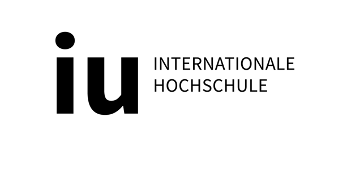
\includegraphics[width=.21\paperwidth]{logos/IU.png}

\begin{center}
\hbox{}
\vfill
{\usesf}
{\huge\bfseries Meine Fallstudie \par}
\vskip 1.8cm
Fallstudie\\[2mm]
\vskip 1cm

{\large\bfseries Markus Haug (<Matrikelnummer>)\\}
\vskip 1.2cm
Wirtschaftsinformatik (B.Sc.)\\
% im Modul\\
ABCDF01 - Kurskürzel\\
\today % TODO: Check Datum
\vskip 3cm
\begin{tabular}{p{3cm}l}
Tutorin: & \usebox{\Tutorin} \\
\end{tabular}
\vfill
\end{center}

\end{titlepage}
%% Titelseite Ende


%%% Local Variables:
%%% mode: latex
%%% TeX-master: "thesis"
%%% End:
 % Titelblatt
\blankpage

%% ++++++++++++++++++++++++++++++++++++++++++
%% Verzeichnisse
%% ++++++++++++++++++++++++++++++++++++++++++
\setcounter{tocdepth}{3}
\tableofcontents % Inhaltsverzeichnis
\blankpage
\listoffigures % Abbildungsverzeichnis
\addcontentsline{toc}{section}{Abbildungsverzeichnis}
\blankpage
\listoftables % Tabellenverzeichnis
\addcontentsline{toc}{section}{Tabellenverzeichnis}
\blankpage
\section*{Abkürzungsverzeichnis}
\addcontentsline{toc}{section}{Abkürzungsverzeichnis}

\begin{acronym}
\acro{lcnc}[LCNC]{Low-Code/No-Code}
\end{acronym}
\label{last-roman-page}% Save last page of this chapter

%% ++++++++++++++++++++++++++++++++++++++++++
%% Hauptteil
%% ++++++++++++++++++++++++++++++++++++++++++
\blankpage
\pagenumbering{arabic}
\section{Einleitung}

Bis zum Jahr 2030 wird der weltweite Fachkräftemangel voraussichtlich insgesamt 82,5 Millionen Fachkräfte umfassen. Insbesondere in der IT-Branche fehlen zahlreiche talentierte Fachkräfte, vor allem Entwickler, um die digitale Transformation eines Unternehmens mit vorantreiben zu können (\cite{grid_dynamics_holdings_inc_software_2022}). Dadurch, dass es für Unternehmen immer schwieriger wird, talentierte professionelle Entwickler einzustellen, stellt dies eines der größten Risiken für Unternehmen dar (\cite{gartner_inc_gartner_2019}).

In den letzten Jahren wurden vermehrt Entwicklungsplattformen auf den Markt gebracht, die sich hauptsächlich dadurch auszeichnen, Anwendungen oder Prozesse mit visuellen Werkzeugen zu erstellen. 
Der Einsatz dieser sogenannten \ac{lcnc}-Plattformen erfordert oft sehr geringe Programmierkenntnisse (\cite[070007-2]{sahinaslan_low-code_2021}). Dies ermöglicht wiederum den Einsatz außerhalb der IT-Abteilung, wodurch erfahrene Anwender aus den Fachabteilungen, Anwendungen selbst erstellen oder Prozesse automatisieren können (\cite[101]{lebens_rise_2021}). 

Diese Anwender werden auch „Citizen Developer“ genannt. Gartner, Inc. (\cite*[][]{gartner_inc_gartner_nodate}) definiert diese im “Information Technology Gartner Glossary” wie folgt:

\begin{adjustwidth}{1.27cm}{0cm}
A citizen developer is an employee who creates application capabilities for consumption by themselves or others, using tools that are not actively forbidden by IT or business units. 
A citizen developer is a persona, not a title or targeted role. They report to a business unit or function other than IT.
\end{adjustwidth}

Durch die aktive Einbeziehung von Citizen Developers in die digitale Transformation entstehen neue Potenziale, aber auch Herausforderungen. 
Folgende Forschungsfragen werden im Rahmen dieser Arbeit beantwortet: 

\begin{itemize}
\item Welche Potenziale eröffnen sich für Unternehmen durch die Nutzung von \ac{lcnc}-Plattformen und wie wirkt sich der Einsatz auf den Mangel von Entwicklern aus? 
\item Welche Maßnahmen sind erforderlich, um die mit \ac{lcnc}-Plattformen einhergehenden Herausforderungen zu bewältigen? 
\end{itemize}

Die Auswirkungen des Einsatzes von \ac{lcnc}-Plattformen auf den Mangel von Entwicklern werden quantitativ erforscht. Darüber hinaus werden IT-Experten und Führungskräfte im Rahmen eines Interviews befragt, welches tiefere Einblicke in die Potenziale und notwendigen Maßnahmen zur Bewältigung potenzieller Herausforderungen in Unternehmen gewähren. Die Ergebnisse werden anschließend ausgewertet und präsentiert. Zum Schluss werden die wichtigsten Inhalte und Erkenntnisse zusammengefasst und es wird ein Ausblick auf mögliche weitere Forschungsthemen gegeben.

\phantomsection
\addtocounter{subsubsection}{1}
\addcontentsline{toc}{subsection}{Problemstellung}

Die Digitalisierung ist in aller Munde. Unternehmen müssen sich immer mehr anpassen, um mit der Konkurrenz Schritt halten zu können.
 % Einleitung
\section{Hauptteil}

\lipsum[1]

\subsection{Titel 1}

Erstes Zitat ist normal mit \parencite[12]{sigfridsson}, das zweite mit "ebenda (ebd.") 
\parencite[78-79]{sigfridsson}, aber nach einer neuen Quelle \parencite[30]{geer} ist es wieder normal \parencite[20]{sigfridsson}.

Dieser Absatz nutzt wieder eine neue Quelle \parencite{nussbaum}.

First citation should be normal \parencite[11]{sigfridsson}, second time with ibidem
\parencite[95]{sigfridsson}, but after a second citation \parencite[282]{geer} it should appear as usual \parencite[2]{sigfridsson}.

\subsection{Titel 2}

Im Abbildung \ref*{fig:logo_iu} in Abschnitt \ref*{pos:logo_iu} wird das Logo der \ac{iu} dargestellt:

\begin{figure}[ht!]
    \label{pos:logo_iu}
    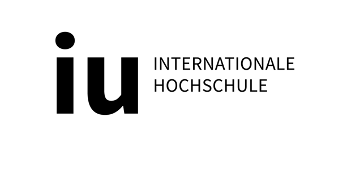
\includegraphics[scale=0.35]{logos/IU.png}
    \caption[Logo der \acs{iu}]{Logo der \ac{iu}}{Quelle: https://iu.de}
    \label{fig:logo_iu}
\end{figure}


\lipsum[7-8]  % Grundlagen
%\include{chapters/analyse}     % Analyse
%\include{chapters/entwurf}     % Entwurf
%\include{chapters/implementierung}    % Implementierung
%\include{chapters/evaluation}        % Evaluierung
%\include{chapters/zusammenfassung}   % Zusammenfassung und Ausblick

\label{last-arabic-page}% Save last page of this chapter

%% ++++++++++++++++++++++++++++++++++++++++++
%% Literatur
%% ++++++++++++++++++++++++++++++++++++++++++
\blankpage

%% Continue page numbering from last roman page
\renewcommand{\thepage}{\roman{page}}% Switch to roman numbering
\edef\intpagevalue{\getpagerefnumber{last-roman-page}}% Retrieve last roman page & convert to arabic
\setcounter{page}{\number\numexpr\expandafter\arabicnumeral\expandafter{\intpagevalue}+1}% Set current page value
\renewcommand{\thepage}{\Roman{page}}% Switch back to arabic numbering

\phantomsection
% set bibliography name
\renewcommand{\bibname}{Literaturverzeichnis}
\addcontentsline{toc}{section}{\bibname}
% \nocite{*} % nur angeben, wenn auch nicht im Text zitierte Quellen 

\begin{flushleft}
% print bibliography
\printbibliography[title=\bibname]
\end{flushleft}

%% ++++++++++++++++++++++++++++++++++++++++++
%% Anhang
%% ++++++++++++++++++++++++++++++++++++++++++
\blankpage

%% Continue page numbering from last arabic page
\renewcommand{\thepage}{\arabic{page}}% Switch to roman numbering
\edef\intpagevalue{\getpagerefnumber{last-arabic-page}}% Retrieve last roman page & convert to arabic
\setcounter{page}{\number\numexpr\expandafter\arabicnumeral\expandafter{\intpagevalue}+1}% Set current page value
\renewcommand{\thepage}{\arabic{page}}% Switch back to arabic numbering

\appendix
%\section{Anhang}

\lipsum[1-2] % Anhang

\end{document}

